% Results

\begin{slide}{Results}
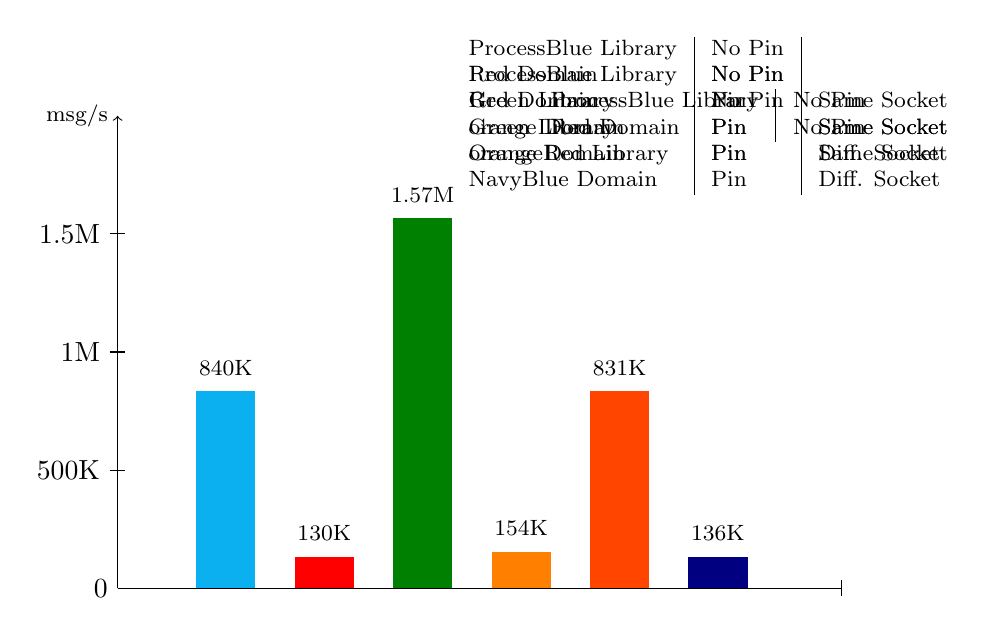
\begin{tikzpicture}

  % No pin
  \onslide<2->{
    % TSSX
    \fill [ProcessBlue] (1, 0) rectangle ++(0.75, 2.5);
    \draw (1.375, 2.8) node {\footnotesize 840K};

    % Domain
    \fill [Red] (2.25, 0) rectangle ++(0.75, 0.4);
    \draw (2.625, 0.7) node {\footnotesize 130K};
  }

  % Same Socket
  \onslide<4->{
    % TSSX
    \fill [Green] (3.5, 0) rectangle ++(0.75, 4.7);
    \draw (3.875, 5) node {\footnotesize 1.57M};

    % Domain
    \fill [orange] (4.75, 0) rectangle ++(0.75, 0.46);
    \draw (5.125, 0.76) node {\footnotesize 154K};
  }

  % Different socket
  \onslide<3->{
    % TSSX
    \fill [OrangeRed] (6, 0) rectangle ++(0.75, 2.5);
    \draw (6.375, 2.8) node {\footnotesize 831K};

    % Domain
    \fill [NavyBlue] (7.25, 0) rectangle ++(0.75, 0.4);
    \draw (7.625, 0.7) node {\footnotesize 136K};
  }

  % Legend
  \onslide<2>{
    \draw (7.5, 6) node {
      \footnotesize
      \begin{tabular}{l | l}
        \legendsquare{ProcessBlue}  Library & No Pin\\
        \legendsquare{Red} Domain & No Pin\\
      \end{tabular}
    };
  }
  \onslide<4>{
    \draw (7.5, 6) node {
      \footnotesize
      \begin{tabular}{l | l | l}
        \legendsquare{ProcessBlue}  Library & No Pin & \\
        \legendsquare{Red} Domain & No Pin & \\
        \legendsquare{Green} Library & Pin & Same Socket\\
        \legendsquare{orange} Domain & Pin & Same Socket\\
        \legendsquare{OrangeRed} Library & Pin & Diff. Socket\\
        \legendsquare{NavyBlue} Domain & Pin & Diff. Socket
      \end{tabular}
    };
  }
  \onslide<3>{
    \draw (7.5, 6) node {
      \footnotesize
      \begin{tabular}{l | l | l}
        \legendsquare{ProcessBlue}  Library & No Pin & \\
        \legendsquare{Red} Domain & No Pin & \\
        \legendsquare{Green} Library & Pin & Same Socket\\
        \legendsquare{orange} Domain & Pin & Same Socket\\
      \end{tabular}
    };
  }

  % Axes (draw here to overdraw bar borders)
  \draw [-|] (0, 0) node [left] {0} -- (9.2, 0);
  \draw [->] (0, 0) -- (0, 6) node [left] {\footnotesize msg/s};

  \foreach \y/\l in {1.5/500K, 3/1M, 4.5/1.5M} {
    \draw (-0.1, \y) node [left] {\l} -- ++(0.2, 0);
  }
\end{tikzpicture}
\end{slide}
